\documentclass{ctexbeamer}
\usetheme{Dresden}
\usecolortheme{spruce}
\usepackage{amsmath, amsfonts, amssymb}
\usepackage{tikz}
\usepackage{listings}
\usepackage{IEEEtrantools}
\special{dvipdfmx:config z 0} % delete this when release
\usetikzlibrary{positioning, arrows.meta, shapes.geometric}
\lstset{basicstyle=\ttfamily}

\title{Processor Arch: Pipelined}
\author{庄嘉毅}
\date{October 2022}

\def\QED{\hfill $\square$}
\def\st{\textrm{s.t.}\,}
\def\imply{\draw[-{Implies[]}, double distance=2pt]}
\DeclareMathOperator{\e}{e}
\newcommand{\ftitle}[1]{\frametitle{\hspace{4ex} {#1}}}
\newcommand{\bfig}[2][1.0]{
    \begin{figure}[hb]\centering\resizebox{#1\columnwidth}{!}{#2}
    \end{figure}
}
\newcommand{\roq}[1]{\rotatebox[origin=c]{-90}{#1}}

\usefonttheme{professionalfonts}
\everymath{\displaystyle}
\linespread{1.5}

\begin{document}

\begin{frame}
    \titlepage
\end{frame}

\section{为什么需要流水线?}
\begin{frame}
    \ftitle{为什么需要流水线?}

    \begin{itemize}
        \item<2- > 顺序结构无法发挥 CPU 的全部性能.
        \item<3- > 以五阶段处理器为例, 处理器在执行一个阶段时,
            其他阶段的电路都处于空闲状态.
    \end{itemize}

    \onslide<3- >\bfig{
        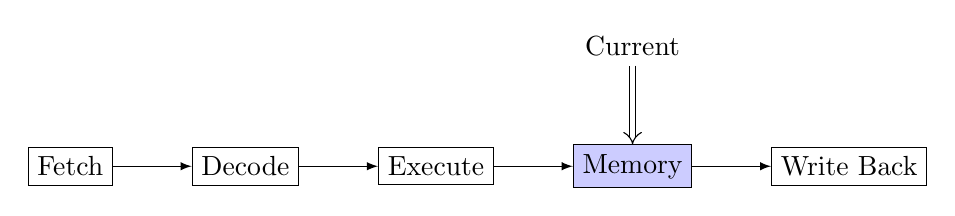
\begin{tikzpicture}
            \node [draw] (A) {Fetch};
            \node [draw, right=of A] (B) {Decode};
            \node [draw, right=of B] (C) {Execute};
            \node [draw, right=of C, fill=blue!20] (D) {Memory};
            \node [draw, right=of D] (E) {Write Back};
            \node [above=of D] (R) {Current};

            \draw[-latex] (A) -- (B);
            \draw[-latex] (B) -- (C);
            \draw[-latex] (C) -- (D);
            \draw[-latex] (D) -- (E);
            \imply (R) -- (D);
        \end{tikzpicture}
    }
\end{frame}

\begin{frame}
    \ftitle{理想的流水线复用}

    \onslide<2- >{每个阶段的电路都在执行一条指令, 如同流水线一样依次进行.}

    \onslide<3- >\bfig{
        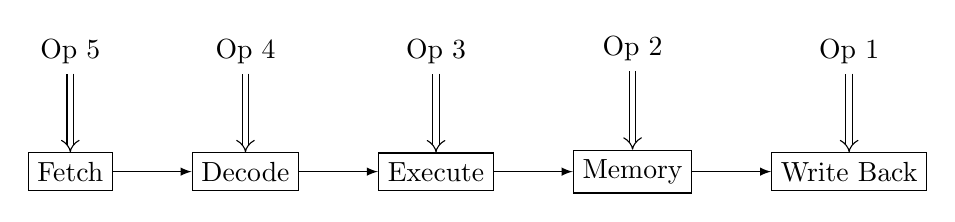
\begin{tikzpicture}
            \node [draw] (A) {Fetch};
            \node [draw, right=of A] (B) {Decode};
            \node [draw, right=of B] (C) {Execute};
            \node [draw, right=of C] (D) {Memory};
            \node [draw, right=of D] (E) {Write Back};
            \node [above=of A] (A1) {Op 5};
            \node [above=of B] (B1) {Op 4};
            \node [above=of C] (C1) {Op 3};
            \node [above=of D] (D1) {Op 2};
            \node [above=of E] (E1) {Op 1};

            \draw[-latex] (A) -- (B);
            \draw[-latex] (B) -- (C);
            \draw[-latex] (C) -- (D);
            \draw[-latex] (D) -- (E);
            \imply (A1) -- (A);
            \imply (B1) -- (B);
            \imply (C1) -- (C);
            \imply (D1) -- (D);
            \imply (E1) -- (E);
        \end{tikzpicture}
    }
\end{frame}

\section{流水线的实现}
\begin{frame}[fragile]
    \ftitle{改造顺序电路}

    \begin{itemize}
        \item<2- > 组合电路与代码不同, 其自身是没有时序保证的.
        \item<4- > 顺序电路的时序是如何保证的?
    \end{itemize}


    \onslide<3- >\begin{columns}
        \begin{column}{.5\linewidth}
            \bfig{
                \begin{tikzpicture}
                    \node (1) at (0, 1) {1};
                    \node (2) at (0, 0) {2};
                    \draw[black] (1, 1.5) rectangle (2, -0.5);
                    \node (ALU) at (1.5, 0.5) {ALU};
                    \draw (1) -- (1, 1);
                    \draw (2) -- (1, 0);
                    \node (3) at (3, 0.5) {3};
                    \draw (2, 0.5) -- (3);
                    \node (4) at (0, -1) {4};
                    \draw[black] (4, 1) rectangle (5, -1.5);
                    \node (ALU) at (4.5, -0.25) {ALU};
                    \draw (3) -- (4, 0.5);
                    \draw (4) -- (4, -1);
                    \node (7) at (6, -0.25) {7};
                    \draw (5, -0.25) -- (7);
                \end{tikzpicture}
            }
        \end{column}
        \begin{column}{.5\linewidth}
            \begin{lstlisting}
int a = 1 + 2;
int b = 4;
int c = a + b;
            \end{lstlisting}
        \end{column}
    \end{columns}
\end{frame}

\begin{frame}
    \ftitle{时序问题}
    \begin{itemize}[<+- >]
        \item 一个逻辑门的输出总是接到另一个逻辑门的输入端.
        \item 电信号传播需要时间, 但无法依赖于此来保证时序.
        \item 在组合逻辑计算完成之后, 如果输入不变, 其状态保持稳定.
        \item 在计算完成之前, 其状态是不稳定的, 不应该使用其结果.
        \item 需要有一个手段来保证稳态是能够对齐的.
    \end{itemize}
\end{frame}

\begin{frame}
    \ftitle{流水线寄存器}
    \begin{itemize}[<+- >]
        \item 寄存器的输出只有收到时钟信号才会改变, 能够起到状态对齐的作用.
        \item 为了在顺序处理器的五个状态之间创造明确的划分,
              需要在每个状态之间加入寄存器.
    \end{itemize}

    \onslide<3- >\bfig{
        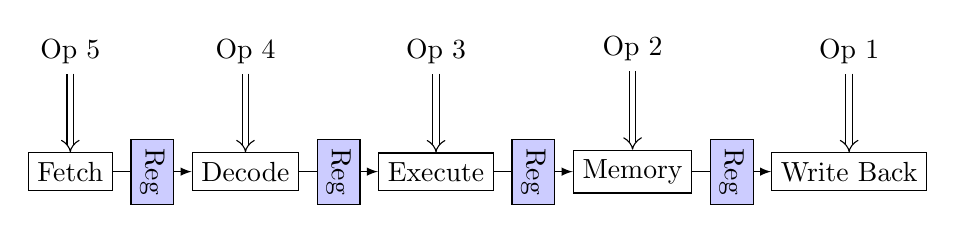
\begin{tikzpicture}
            \node [draw] (A) {Fetch};
            \node [draw, right=of A] (B) {Decode};
            \node [draw, right=of B] (C) {Execute};
            \node [draw, right=of C] (D) {Memory};
            \node [draw, right=of D] (E) {Write Back};
            \node [above=of A] (A1) {Op 5};
            \node [above=of B] (B1) {Op 4};
            \node [above=of C] (C1) {Op 3};
            \node [above=of D] (D1) {Op 2};
            \node [above=of E] (E1) {Op 1};

            \draw[-latex] (A) -- (B) node[midway, draw, fill=blue!20!white] {\roq{Reg}};
            \draw[-latex] (B) -- (C) node[midway, draw, fill=blue!20!white] {\roq{Reg}};
            \draw[-latex] (C) -- (D) node[midway, draw, fill=blue!20!white] {\roq{Reg}};
            \draw[-latex] (D) -- (E) node[midway, draw, fill=blue!20!white] {\roq{Reg}};
            \imply (A1) -- (A);
            \imply (B1) -- (B);
            \imply (C1) -- (C);
            \imply (D1) -- (D);
            \imply (E1) -- (E);
        \end{tikzpicture}
    }
\end{frame}

\begin{frame}
    \ftitle{流水线寄存器}
    \onslide<1- >{顺序相连的寄存器, 形成了逻辑上的队列结构.}
    
    \foreach \t[evaluate=\t as \p using {int(\t+1)},
        evaluate=\t as \u using {int(\t-1)},
        evaluate=\t as \v using {int(\t-2)},
        evaluate=\t as \w using {int(\t-3)}] in {1,...,4}{
            \onslide<\p- >\bfig[0.8]{
                \begin{tikzpicture}
                    \node [draw, fill=blue!20] (I) at (0, 0) {Inc};
                    \node [draw] (A) at (2, 0) {Reg};
                    \node [draw] (B) at (4, 0) {Reg};
                    \node [draw] (C) at (6, 0) {Reg};
                    \node [draw] (D) at (8, 0) {Reg};
                    \draw[-latex] (I) -- (A) node[midway, above] {\ifnum\t>0 \t \else \fi};
                    \draw[-latex] (A) -- (B) node[midway, above] {\ifnum\u>0 \u \else \fi};
                    \draw[-latex] (B) -- (C) node[midway, above] {\ifnum\v>0 \v \else \fi};
                    \draw[-latex] (C) -- (D) node[midway, above] {\ifnum\w>0 \w \else \fi};
                    \node (E) at (9, 0) {$\cdots$};
                \end{tikzpicture}
            }
        }
\end{frame}

\begin{frame}
    \ftitle{流水线寄存器}
    \begin{itemize}
        \item<1- > 流水线寄存器里面有什么?
              \onslide<2- >\begin{itemize}
                  \item 上一个阶段的计算结果.
                  \item 之前的阶段接收的值, 没有经过计算, 但会在之后阶段用到.
              \end{itemize}
        \item<3> 依赖时序的数据连接不会越过流水线寄存器.
    \end{itemize}
\end{frame}

\begin{frame}
    \ftitle{实例:自增电路}
    \onslide<1- >{一个自增电路, 每个时钟周期输出值加1.}
    \onslide<2- >\bfig[0.6]{
        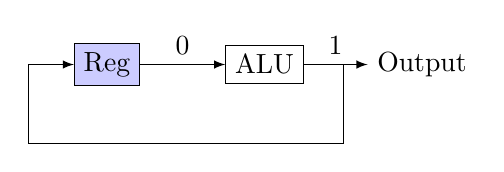
\begin{tikzpicture}
            \node [draw, fill=blue!20] (I) at (0, 0) {Reg};
            \node [draw] (A) at (2, 0) {ALU};
            \node (O) at (4, 0) {Output};
            \draw[-latex] (I) -- (A) node[midway, above] {0};
            \draw[-latex] (A) -- (O) node[midway, above] {1};
            \draw[-latex] (3, 0) -- (3, -1) -- (-1, -1) -- (-1, 0) -- (I.west);
        \end{tikzpicture}
    }

    \onslide<3- >{推广: PC 预测.}

    \onslide<3- >\bfig[0.6]{
        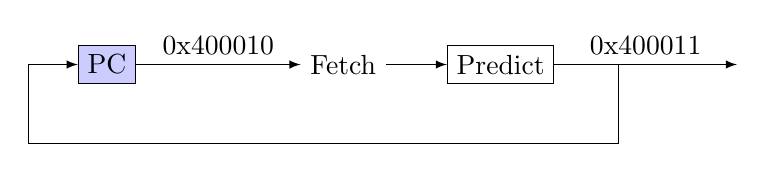
\begin{tikzpicture}
            \node [draw, fill=blue!20] (I) at (0, 0) {PC};
            \node (O) at (3, 0) {Fetch};
            \node [draw] (A) at (5, 0) {Predict};
            \draw[-latex] (I) -- (O) node[midway, above] {0x400010};
            \draw[-latex] (O) -- (A);
            \draw[-latex] (A) -- (8, 0) node[midway, above] {0x400011};
            \draw[-latex] (6.5, 0) -- (6.5, -1) -- (-1, -1) -- (-1, 0) -- (I.west);
        \end{tikzpicture}
    }
\end{frame}

\section{流水线冒险}
\begin{frame}
    \ftitle{流水线冒险}
    \begin{itemize}
        \item<2- > 数据冒险
              \begin{itemize}
                  \item<3- > 下一条指令需要某一个寄存器参与运算, 但上一条指令更新了这个寄存器.
              \end{itemize}
        \item<4- > 控制冒险
              \begin{itemize}
                  \item<5- > 下一条指令是条件跳转, 需要上一条指令确定条件码.
                  \item<6- > 下一条指令是 \texttt{ret}, 需要访问内存确定下一条指令的地址.
              \end{itemize}
    \end{itemize}
\end{frame}

\begin{frame}
    \ftitle{数据转发}
    \begin{itemize}
        \item<2- > 前后两条指令的执行在流水线中相差一个阶段.
        \item<3- > 寄存器数据的读取发生在译码阶段, 此时上一条指令正在执行阶段.
        \item<4- > 如果寄存器的新值在执行阶段时就能够计算出来
              (例如 \texttt{add} 这样的算数指令),
              那么就可以把结果直接传递给下一条指令.
        \item<5- > 如果寄存器的新值在执行阶段得不到
              (例如 \texttt{movq (\%rax), \%rax}),
              则无法进行数据转发.
    \end{itemize}
\end{frame}

\begin{frame}
    \ftitle{分支预测}
    \begin{itemize}
        \item<2- > 对于 \texttt{jxx} 指令, 倾向于认为条件成立.
              \begin{itemize}
                  \item<3- > 其他跳转策略: 向低地址跳转.
                  \item<4- > 原理: 大量的条件跳转发生在循环中, 而循环在未结束时往往向低地址跳转.
              \end{itemize}
        \item<5- > 对于 \texttt{ret} 指令, 可以使用硬件栈进行预测, 或者放弃预测.
    \end{itemize}
\end{frame}

\begin{frame}
    \ftitle{暂停与取消}
    \begin{itemize}
        \item<2- > 发生加载/使用冒险而暂停时, 关闭PC寄存器和译码寄存器的写入,
              向执行寄存器写入 \texttt{bubble}/\texttt{nop}.
              \begin{itemize}
                  \item<3- > 关闭写入: 使电路不断重复执行同一条指令的某个阶段.
              \end{itemize}
        \item<4- > 遇到 \texttt{ret} 指令而暂停时, 之后的三个周期里,
              取值阶段的行为改为直接向译码寄存器写入 \texttt{bubble}/\texttt{nop}.
        \item<5- > 发生取消时, 向译码和执行寄存器写入 \texttt{bubble}/\texttt{nop}.
              \begin{itemize}
                  \item<6- > 不需要关闭寄存器写入, 因为这两种情况都在等待新的PC.
              \end{itemize}
    \end{itemize}
\end{frame}

\begin{frame}
    \ftitle{异常处理}
    \begin{itemize}
        \item<2- > 异常发生后, 需要保证异常指令之前的指令能继续走完流水线,
              同时避免异常指令之后的指令的副作用.
        \item<3- > 流水线寄存器中的 \texttt{stat} 状态位用于标记异常.
        \item<4- > \texttt{stat} 走出流水线时, 实际引发异常.
        \item<5- > \texttt{stat} 在流水线内时, 屏蔽其之后的指令的副作用(访存/写回/条件码).
    \end{itemize}
\end{frame}

\section{性能分析}
\begin{frame}
    \ftitle{性能分析}
    \begin{itemize}
        \item<2- >$\mathrm{CPI}$: 每指令周期数.
        \item<2- >$\mathrm{IPC}$: 每周期指令数.
    \end{itemize}    

\end{frame}

\end{document}
